\PassOptionsToPackage{dvipsnames,svgnames,x11names}{xcolor}
\documentclass[a4paper]{article}
\usepackage[T1]{fontenc}
\usepackage[ngerman,british]{babel}
\usepackage{authblk}
\usepackage{csquotes}
\usepackage[alldates=iso,seconds=true,sorting=none]{biblatex}
\usepackage{graphicx}
\usepackage[margin=2.5cm]{geometry}

\DeclareUnicodeCharacter{200B}{{\hskip 0pt}}

\usepackage{libertine}
\usepackage{orcidlink}
\usepackage{rorlink}
\renewcommand\Affilfont{\small}

\usepackage{hyperref}
\urlstyle{same}
\usepackage{xspace}
\usepackage{caption,tikzpagenodes,ifthen}

\usepackage{mdframed}

\newcommand*{\eg}{e.\,g.,\xspace}
\newcommand*{\ie}{i.\,e.,\xspace}

\hypersetup{%
  %pdftitle={},
  %pdfkeywords={},
  colorlinks=true,
  linkcolor={darkgray},
  filecolor={Maroon},
  citecolor={Blue},
  urlcolor={Blue},
}

\addbibresource{bibliography.bib}
\addbibresource{positionpaper.bib}
\setcounter{biburllcpenalty}{100}

\title{Developing central Research Software Engineering units in German research institutions}

% The file contributors.tex is automatically generated by running contributors.py.
% Changed within will be OVERWRITTEN.
% For changes to the tex template, change contributors.tex.j2.
% For changes to the author information, change contributors.yml.
%
\author[]{Markus Ankenbrand}
\author[]{Bernd Flemisch}
\author[5]{Florian Goth}
\author[3]{Jean-Noël Grad}
\author[2]{Dominic Kempf}
\author[4]{Jan Linxweiler}
\author[]{Axel Loewe}
\author[](Leyla Jael Castro)
\author[](Philipp S. Sommer)
\author[1]{Frank Löffler}
\author[1]{Philipp Matthias Schäfer}
\author[]{Alexander Struck}
\affil[1]{Competence Center Digital Research, Michael Stifel Center Jena, Friedrich Schiller University Jena, Jena, Germany}
\affil[2]{Heidelberg University, Scientific Software Center, Germany}
\affil[3]{Institute for Computational Physics, University of Stuttgart, Germany}
\affil[4]{Technische Universität Braunschweig, Germany}
\affil[5]{Institute for Theoretical Physics and Astrophysics, University of Würzburg, Germany}


\date{\today}

\begin{document}

\maketitle

\abstract{%
This position paper urges decision makers in Germany to establish central Research Software Engineering (RSE) units within their institutions.
The focus is not put primarily on the establishment of RSE services in general, as this has been done already elsewhere.
Instead, we highlight central RSE units.
Motivation for their existence is discussed, underpinned by working examples both in neighbouring fields as well as outside of Germany.
The heart of this paper is a vision of a central RSE unit, its structure, and the definition of nine core support modules such a unit may provide.
An initial survey finds that there is considerable diversity within the module distribution, even within the few considered groups.
We discuss initial observations on possible clusters, but further studies are needed.
Finally, we discuss realisation strategies.
While this paper focuses mostly on the German academic environment, some general strategies should also apply elsewhere.
}

\section{Introduction}
Research software has been written and used for decades in an increasing range of disciplines.
It has been established that most research requires research software for its results~\autocite{Hannay2009, Hettrick2015}.
To solve pressing research challenges, better software is crucial~\autocite{Goble2014}.
During the past decade, research software gained ever-growing attention and is becoming accepted as a research result in its own right.

The number of people developing software in academia is continuously rising~\autocite{Hannay2009, Hettrick2015}.
Research software engineering encompasses creating, adapting or maintaining research software.
It also includes consultation and training with the aim to enable researchers to some of these tasks themselves~\autocite{goth_foundational_competencies_2024}.
These actions are very diverse and so are the environments they are performed in.
This position paper focuses on groups of research software engineers that provide their services for an entire research organisation or at least a substantial part of it.

We advocate the establishment and support of dedicated, central RSE groups in German research organisations, with clearly defined tasks, points of contact, and, in particular, sustained funding, for the benefit of all researchers in their organisation.
Similar initiatives have been formed in other national contexts (see~\autocite{barkerkatz2024,martin2023} and references therein).
We provide an overview of the various tasks these teams have and discuss potential realisation strategies, learning from already existing RSE units.

Depending on the national research environments and processes that readers are familiar with, the notion of the terms \emph{software} and \emph{research} might differ.
The term “research software” has also no single definition within the community.
Therefore, to avoid ambiguities, we list the definitions that we use in this document:
\paragraph{Software}
Source code, documentation, tests, executables, and all other artefacts that are created during the development process and that are necessary to understand its purpose.
\paragraph{Research software}
Foundational algorithms, the software itself, as well as scripts and computational workflows that were created during the research process or for a research purpose, across all domains of research.
This definition is broader than in~\autocite{FAIR4RS} and is the outcome of a recent discussion in~\autocite{Gruenpeter2021}.
\paragraph{Research software engineers}
People who create or improve research software and/or the structures that the software interacts with the computational ecosystem of a research domain.
They are highly skilled team members who may also conduct their own research as part of their role.
However, we also recognise RSEs who have chosen to focus on a technical role as an alternative to a traditional research role.
\paragraph{Researchers}
We call RSEs who are members of the RSE hub (see below) dedicated RSEs.
RSEs who are members of a research group are called embedded RSEs.
RSEs might also be researchers.
However, for the lack of a proper term and to avoid many “non-RSE researchers” within the text, we will use the term “researchers” to refer to all non-RSEs involved in research or in research supporting organisations such as in, \eg{} libraries.
Another way to define the group of researchers are all people who at most very occasionally perform RSE actions.
\paragraph{RSE Hub}
This is our general term for the central RSE team throughout this paper.
These RSE Hubs can take the form of, \eg{} full RSE units, smaller RSE groups, Open Source Program Offices (OSPOs), virtually across multiple units or combined under single leadership, depending on the environment of the hosting research organisation.
All of these implementations are considered, taking into account the large variety of research environments in Germany, which include not only universities, but also research consortia and other research performing organisations.
We use the term central \emph{RSE unit} interchangeably with the term \emph{RSE hub} even though for large federated research organisations there might be a more complex arrangement such as a network of RSE hubs.

\section{Motivation for central RSE units}
\begin{quotation}
      \noindent \textit{Better Software, Better Research}\\(Mission statement of the UK Software Sustainability Institute)
\end{quotation}

The quote above is the shortest possible summary of this chapter: most if not all motivation to provide RSE services stems from the goal of improving research.
Tasks that Research Software Engineers (RSEs) perform include training, \eg{} to improve the quality of code produced by researchers~\autocite{Ostlund2023}, consultation services, \eg{} regarding frameworks or algorithm selection, and the development of existing or new software.
For an overview of typical tasks of RSEs and the competencies required, see~\autocite{goth_foundational_competencies_2024}, especially section\ 4.4:\ “RSE tasks and responsibilities”.

Research software is getting increasingly complex.
This is partly because the scientific problems being tackled using software are getting bigger.
However, the software is also expected to be reliable, secure and easy to use.
Handling this increased complexity whilst ensuring timely delivery requires dedicated RSEs in central RSE units.

\subsection{Pooling: a necessary ingredient}
The main focus of this paper lies on central RSE teams since the benefits of RSEs to research in general are described elsewhere, \eg{} in~\autocite{Anzt2021}.
The main advantages of central RSE units all stem from the pooling of resources.
There are at least three aspects to RSE pooling that research institutions can benefit from: funding, diverse knowledge, and a central point of contact.
First, pooling of \textbf{funding} allows organisations to invest in building up institutional knowledge by supporting RSEs to become experts.
A central RSE team on long-term contracts will act as a knowledge hub due to their accumulated experience in and support of several disciplines as well as established contacts within the organisation.
This is comparable to commercial/industry R\&D departments or so-called inhouse consulting~\autocite{Grima_2011}, where key software architects and developers establish a knowledge hub that can be consulted by project teams as necessary.
Subject matter experts like software architects, database administrators and other tooling specialists are organised centrally and share their knowledge with members of decentralised projects.
It makes economic sense to organise such staff centrally, since not every project has a need for a full-time specialist or can afford one over an extended period of time.
Most academic research organisations have established centralised tooling, \eg{} storage or High-Performance-Computing\ (HPC), but only a few consider software development and consultancy a relevant service yet.

A second and equally important aspect to pooling RSEs is that of \textbf{diverse knowledge}.
RSE units act as knowledge hubs in a network of academic developers within an organisation~\autocite{Elsholz2006}.
Groups of RSEs with tasks spanning the entire organisation necessarily have to offer diverse knowledge.
Obtaining this diversity of knowledge and experience can also be a challenge, but once it has been established it quickly becomes an asset to the organisation.
RSEs in centralised groups are interdisciplinary specialists.
They are interdisciplinary due to their broad experience by working on diverse research topics and their ability to apply a diverse set of research methodologies.
At the same time they are specialists concerning research software and how it can best improve research.
They are assumed to be able to suggest the most appropriate tools/frameworks and design or architecture patterns for certain research challenges.
Their diversity in skills (languages, frameworks, front/back-end, UX, management) is welcomed, especially for short-term needs in projects.
This will improve the chances of a project being successfully completed in a timely manner.
That means a central RSE unit has more RSE competencies than any individual research group in the institution.
This allows members of that unit to bring in new ideas or transfer them from other collaborations to these groups.
Furthermore, by centralising RSE expertise, the unit benefits from economies of scale, making it feasible to handle also less frequently needed tasks across multiple groups.
This synergy broadens the scope of possible software-based solutions while distributing costs and resources more efficiently.

The third aspect to pooling RSEs is visible most of all from a users perspective: a \textbf{single, central point of contact} for digital challenges is valuable to researchers, whose first problem often is not knowing whom to contact, partially because while they know what they want, they might not know what they need.
A central RSE team can, due to its proximity to research, much better listen to the wishes expressed by researchers and then help formulate needs and act as a channel to either fulfil them themselves or reformulate and redirect the request.
The results are increased research speed and quality and, with that, a higher reputation of the entire research organisation.

Working in a research institution is very stimulating.
However, an embedded RSE can feel very lonely when they do not have anybody to discuss technical problems.
A central RSE unit also provides a social space for RSEs where this exchange can easily happen.

\subsection{Pooling: an already tested idea}
The idea to pool resources in specific areas within an organisation is not new.
In industry, software engineering underwent a similar transition about 20 years ago, with the creation of specialised, central software development units.
In an example from academia, similar arguments can and have been made for research data support.

\subsubsection{Research data management}
Both data and software play a fundamental role in almost all of research.
Over the past decades, Research Data Management (RDM) has evolved into a topic of national interest with NFDI\footnote{Nationale Forschungsdateninfrastruktur: the national research data infrastructure in Germany} consortia for all disciplines and a research data law.
Federal state RDM initiatives\footnote{\url{https://forschungsdaten.info/fdm-im-deutschsprachigen-raum/deutschland/}} have established the topic further and provide regional training, networking and other supporting services.
Many research organisations have set up established central RDM groups that support research projects in all aspects from grant proposals to hands-on support and maintaining Data Management Plans (DMPs).
Funding agencies acknowledge the importance of research data and have started to make RDM mandatory in research projects.

The most recent funding guidelines suggest to have “data stewards” in data-driven research.
Such experts are to be employed in advanced research projects like “Collaborative Research Centres” (CRC)\footnote{Sonderforschungsbereich (SFB)} or “Clusters of Excellence”\footnote{Cluster der Exzellenzinitiative}.
These data experts support research projects in several aspects including DMPs, grant applications, data availability for journal publications, compliance, FAIRification and more.
Similarly, central RSEs will encourage other RSEs to publish software with rich metadata and will support journal publications with code submission requirements.
With the increasing recognition of software as a research product, it is easy to see how projects will require and benefit from support in research software management in the near future.

Due to the similar nature of both, data and software, and their importance in today's digital research, it is reasonable to expect a similar trajectory in the development of research software as a topic, as we have witnessed for research data.

\subsubsection{Existing RSE efforts}
Some organisations already have central RSE teams.
The field of RSE teams in Germany is currently poorly mapped and very diverse.
It includes groups with responsibilities across institutions like the Helmholtz HIFIS group~\autocite{haupt_hifis_consulting_2021, HIFIS}, but mostly groups with responsibilities local to their institution.
Their anchoring within institutions also differs:
Some are part of an existing interdisciplinary research institution (like the Scientific Software Center in Heidelberg~\autocite{keegan_ssc_whitepaper,HeidelbergSSC}).
Others are part of the central university research support infrastructure and are goverened by the institutional leadership (like the Competence Center Digital Research (zedif) in Jena~\autocite{zedifUniJena}).
Yet others have a project character, like Suresoft in Braunschweig~\autocite{Blech2022,SURESOFTLink}.
Another national pioneer is the Göttingen State and University Library where RSE services are part of the library-service portfolio.

Most of these groups, or at least their RSE services, are still relatively young.
However, some groups can already report a remarkable increase in software quality, better grant applications, less brain drain and overall better employee satisfaction levels~\autocite{schimavoigt2023}.
RSE services which benefit all disciplines/departments may represent a unique selling point for organisations competing for the brightest minds.

Besides institutions, there are also other communities related to RSE\@.
The HPC community, arguably a sub-community of the RSE-community, has a history of offering training and consulting to prospective and active users of the hardware they support.
National Competence Centres~\autocite{EuroCCWeb} form a network of HPC-RSE consulting groups to share expertise with academic and industry actors~\autocite{eurocc_success_stories_2023,eurocc_success_stories_2024}.

While we focus on Germany in this paper, it is beneficial to review how other countries approach research software.
In the UK, which we choose as example for being the oldest in terms of RSE, many universities started initiating dedicated RSE units about a decade ago~\autocite{Crouch2013, KDL}.
The successful establishment of these units is a role model for similar research performing organisations worldwide.
A range of already existing RSE units in the UK can be seen on this (incomplete) map: \url{https://society-rse.org/community/rse-groups/}.
In the UK, it is common for grant applications to include software development in their budget.
This allocated money can then be utilised to delegate/dispatch a central RSE person or group into a research project for a few weeks or months as necessary.

\subsection{External expectations}

Some of the latest DFG grant application templates (\eg{} the strategy of excellence~\autocite{DFG_ExStra130}) require discussion of both, data \emph{and} software management (in line with their GWP guidelines~\autocite{dfg_gsp}).
In addition, as dedicated DMPs have become mandatory in several funding calls~\autocite{FDM_Info_FDM}, we expect to see a similar development for Software Management Plans (SMPs) in the future.
As of today, they are already recommended~\autocite{FDM_Info_SMP}.

Policies for research software management and guidelines involving responsible research practices detailing software handling are the precursors for a research software engineering environment.
See for example position papers by
 the Helmholtz Open Science Office~\autocite{Helmholtz2019a,Helmholtz2019b},
 the AllianzInitiative~\autocite{Konrad2021},
 the DLR~\autocite{Schlauch2018b},
 the University Utrecht~\autocite{Utrecht2016b},
 and the German Research Council~\autocite{dfg_gsp}.

Another development taking place worldwide is the encouragement of authors to submit both, data and software, for peer review.
As an example, the journal “Nature” initiated such a policy\footnote{\url{https://www.nature.com/nature-portfolio/editorial-policies/reporting-standards}} in 2018~\autocite{Nature2018}.
RSE groups are able to offer researchers consulting tailored to their specific needs on how to implement and document those policies.
This is especially relevant in the context of reproducibility of software-based research.

The global FAIR movement originated from RDM and widened their focus to include research software.
However, it also has become clear in that process that software is not “just another type of data” and that the FAIR principles are not sufficient for software.
The FAIR principles for Research Software (FAIR4RS)~\autocite{ChueHong2022} have been adopted worldwide~\autocite{Barker2024}, including the German Ministry of Education and Research (BMBF) and the German Research Foundation (DFG).
The rather complex assessment of FAIRness~\autocite{Wilkinson2023,FAIRmaturity} has also widened from data to software~\autocite{Lamprecht2020}.

\section{Vision}%
\label{sec:vision}

In this section, we describe our vision for central RSE units at research institutions in Germany.
For our purposes, the term “institutions” is used broadly to include universities, other colleges, associations like Max-Planck, Helmholtz, Fraunhofer, or Leibniz, as well as other research-performing organisations.
They show a wide variety in organisational structure as well as internal scientific diversity.
Thus, there can be no single optimal blueprint for such an RSE unit for all research institutions in Germany.
We instead describe modular components that can be combined for the respective local environment.

We have identified nine modules that can make up an RSE unit.
In practice, most RSE units will only support some of these modules, and different RSE units will focus on different sets of modules.
Thus, it is likely that no two RSE units will be, or need to be, alike.
However, these nine modules, along with their assigned weights (indicating relative importance), form a simple model of an RSE group.
This provides both a quick overview of an individual group as well as a way to compare groups.
The nine modules are described below.

\subsection{Module 1: Foster a local Network of RSEs}%
\label{sec:network}

One of the core responsibilities of an RSE unit is to act as a coordinator of RSE activities within the institution.
Research software is an integral part of modern research.
There are, therefore, researchers in every institution that at least sometimes perform the tasks of an RSE\@.
We call these RSEs embedded RSEs.
These RSEs typically work isolated from similar RSEs in other groups within the same institution.
The central RSE unit together with the embedded RSEs form a hub and spokes network.

Connecting embedded RSEs has multiple positive effects, both for them as well as for the organisation:
It will enable them to learn from others in similar situations and to support each other.
Embedded RSEs can ask a central RSE unit for advice on specific problems.
They can also pass some tasks to the central RSE unit if they lack the knowledge or resources to solve those themselves.
Contact with the central RSE unit also helps RSEs to professionalise their software-related work, which will directly benefit not only themselves but also their research groups.
Additionally, the networking opportunities allow the distribution of knowledge about tools and resources within the network.
Information also flows from the embedded RSEs to the central RSE unit allowing it to discover common requirements and opportunities to centralise some services.

How an RSE unit realises this task will depend heavily on its environment and resources.
We only mention a few examples here for inspiration, with the explicit claim of incompleteness:
talks, seminars, workshops, hackathons, as well as informal meet-ups all facilitate establishing a local network of RSEs.
As a foundation, a central RSE unit employs experienced RSEs, mostly at the post-doctoral level, who are not only expert software engineers and scientists, but also good communicators with the ability to work in interdisciplinary teams.
At least a core of a central RSE unit's employees need to have permanent contracts to be able to offer that deep expertise that requires years of experience.
Moreover, an onboarding process can serve as an entry point for new RSEs, whether in the central RSE unit or as an embedded RSE, into an institution's network.
This gives an opportunity to gauge how the new colleague can benefit from the RSE unit's teaching services and whom they might want to network with based on their planned work.
Similarly an off-boarding process can help to make sure that all acquired knowledge that is relevant to the institution is passed on to someone else, even if possibly not within the specific research group.

\subsection{Module 2: Consultation Services}%
\label{sec:consultation}

With the majority of researchers being self-taught programmers~\autocite{Carver2013}, there is a huge demand for expertise on how to develop better research software.
Here, “better” can refer to a number of quality metrics such as correctness, reproducibility, maintainability, extensibility, usability, portability, interoperability, performance or scalability~\autocite[Chapter 16]{Schulmeyer2008}.

In order to raise the quality standards for research that is based on research software, it is of great importance for research institutions to provide access to such expertise with a low barrier to entry.
The hub is a natural place to provide this central service.
There are a number of scenarios where RSE consultation services differ strongly in scale and format.
We mention a few of these in the following.
“Walk-in” consultations on any research software related aspect that are open to researchers of all career levels are a great introduction to the hub's RSE services and are offered by almost all RSE units already established (see, \eg{} data in Section~\ref{sec:existing} or~\cite{Katz2019}).

A larger scale format for RSE consultation services could be that a research project regularly meets with an RSE in order to coordinate the research software efforts done in the research project.
This format enables valuable feedback cycles between researchers and RSEs and allows RSEs to guide the project towards successful software engineering best practices without overloading the researchers with information at a walk-in consultation.
When an RSE unit carries out many of these project consultations, they will gather valuable experiences in transferring RSE knowledge to practitioners.
An RSE hub puts these experiences into institutional memory, allowing for better RSE practice in the future.

RSE consultation services also have a positive impact on grant proposal quality.
Many proposals critically depend on research software to be developed and the requirements of funding agencies with respect to research software are growing and will continue to do so.
Similar to dedicated RDM units that provide institutional support for data management plans, the RSE hub can support researchers by providing expertise with software management plans and the software engineering best practices required by these plans.
Consultation services that are already involved in the proposal phase are expected to lead to an improved research workflow and thereby to better research.
This in turn leads to improved proposal acceptance rates, thereby amortising the initial investment into RSE units.


\subsection{Module 3: Development Services}%
\label{sec:development}

There is a huge demand for the development and customisation of research software tailored to the needs of specific research projects.
In many cases this can be achieved by educating researchers to write their own software according to RSE best practices.
Bringing in expert RSEs to deal with the development of complex research software frees up the researchers to focus on research.
In these cases, RSE development services are a great opportunity that can have a huge impact on the digitisation of science at a research institution.
Similar to consultation services, this service can be offered at multiple scales.

Many times, even a small effort of a skilled RSE can have a huge impact on a research project that requires dedicated research software development.
With the impact of these projects being usually very high, realising as many of them as possible gives a great boost to the research institution.
Many existing RSE units (\eg{} Manchester, Heidelberg) offer this type of small scale service free of charge and use it to promote their services within the institution.

For research projects requiring more substantial software development resources, an RSE unit could --- either through central or embedded RSEs --- provide the required developer capacity.
This is especially relevant if the researchers hired for the research projects do not have the required software development skills and the volume of the development is too small to hire a dedicated developer.
Depending on the scale of the involvement, the RSE unit can either be included into the grant proposal via a co-PI or as an internal service provider.

If the research within an institution heavily relies on specific pieces of software, it is of vital importance for the long term success of the institution to sustain these pieces of software.
Relying on a workforce that is subject to academic labour turnover poses the risk of knowledge loss and incurs a significant overhead due to the need to constantly search for and then retrain new staff.
If the development is done in an RSE unit with long-term contracts, institutional memory about critical research software infrastructures can be created and the long term availability of these infrastructures can be improved.
This applies both to domain-specific research software (\eg{} simulation frameworks widely used throughout the institution)
  and to domain-agnostic software and data infrastructure (\eg{} Jupyter, workflow management systems, data repository software).

While all of the above development services can be flexibly performed either at the central RSE unit or by embedded RSEs, there are advantages of having a hub in the process:
It allows building up highly specialised technical expertise with a long-term perspective and reuse it across the entire institution.
Examples of topics that would benefit from such expertise pooling are, \eg{} mobile app development and UI/UX development.

RSE units that offer development services at all scales have proven to be a success story at many research institutions and have rapidly grown in size due to the influx of third party funding.
Notable examples~\autocite{Katz2019} are, \eg{} Manchester~\autocite{Sinclair2022}, Notre-Dame~\autocite{NotreDame2025}, Stanford~\autocite{Stanford2025}, Princeton~\autocite{Princeton2025, Cosden2022a}.

\begin{mdframed}
\textbf{Success Story:} The University of Manchester Software and Data Science group has successfully established specialised development services within their institution:
The “Mobile Development Service” \autocite{manchester_mobile} team consists of RSEs that focus solely on developing and deploying mobile apps.
Without a central RSE unit to anchor such specialised expertise, it would be difficult to establish such a service.
Also, having this expertise centralised allows for synergies in the deployment procedure for mobile apps:
The RSE unit can create institutional accounts with the app stores and manage the time-consuming deployment process including hard-to-setup procedures like code signing.
Besides the technical benefits of this central deployment procedure, the institution benefits from the increased visibility and the ability to build a brand with its technological output.
\end{mdframed}

\subsection{Module 4: Teaching Services}%
\label{sec:teaching}

A central RSE unit can provide or organise training for researchers and embedded RSEs.
This can replace self-education for foundational software development skills and provide a basis from which researchers can continue to learn more specialised skills guided by experts of the central RSE unit.
Since teaching material for foundational software development skills is freely available,
  the tasks remaining for a central RSE unit are to adapt the material to local requirements as well as to organise and hold courses and workshops.

For more complex software development projects, a central RSE unit can offer individual training.
In both cases, the expert RSEs from the central RSE unit can pass on their knowledge precisely adapted to the concrete needs of those that they support.
Finally, in organisations that educate RSEs, members of a central RSE unit may contribute to the curriculum of the institutional study programmes and teach corresponding courses.

\subsection{Module 5: Create a Network of Institutional Partners}%
\label{sec:partners}

Within a research institution, a lot of groups or departments touch the topic of research software one way or another.
However, their coverage of RSE-related needs of researchers is often limited and their main responsibilities are diverse and typically lie elsewhere.
This is one of the main arguments for the creation of dedicated RSE units.
However, it also shows the necessity for an RSE unit to closely interact with those partners.

In the following, we describe groups or units that can typically be found within academic organisations, their focus, and how we envision their collaboration with an RSE unit.
However, note that as research organisations can differ widely from one another, so can the tasks and even existence of these entities.
Arguments and conclusions below have to be adapted to specific circumstances when applying them to specific environments.

All research institutions in Germany can use the services provided by a central \textbf{IT unit} in one form or another.
The central IT unit typically looks after common compute and storage infrastructure in data centres and associated network infrastructure.
They also provide software services such as Email, web services, and databases, and administer standard desktops and laptops (at least for administrative staff).
Research software often has to work within the environment provided by the IT unit.
A central RSE unit can help researchers adapt their software to run on central services where necessary.
RSEs can also work with central IT staff to provide IT infrastructure well suited for research projects.
Usually, this requires a level of engagement and understanding of both the underlying research concepts and IT infrastructure that the staff of the IT unit or the researchers each cannot provide alone.

If available, a second important partner is a scientific \textbf{library}, which has already gained tasks much beyond the preservation and organisation of publications on physical paper for quite some time.
Besides digital forms of rather traditional publications, these more and more include digital data and recently also software publications, their discovery and citation.
With the dedicated help of RSEs, research software can be enabled to be added to the organisational bibliography, facilitating internal reporting.
At the same time, through collaboration with the library, the RSE group can address the first two letters of FAIR:\@ Findability and Accessibility.

Both RSE and RDM units provide research-oriented services that are supporting digital research, covering different aspects of the research cycle.
They need to collaborate directly because research software both consumes and produces research data.
Requests for support on digital research therefore often touch both aspects, RSE and RDM\@.
Thus, a close collaboration between RSE and RDM groups helps everyone: both RSE and RDM groups by being able to offer a more comprehensive service than when working alone, as well as the researcher, who benefits from receiving this single coordinated service, instead of dealing with two independent entities.
The question whether RSE and RDM should be located in two separate groups or should be combined in one common group is intentionally left open, as the answer depends on local, pre-existing circumstances.

Some research institutions host a dedicated \textbf{HPC group} which may or may not be part of the central IT unit.
HPC is an RSE-related field, so HPC groups might already provide training, consulting and funding opportunities in this area.
At the same time, HPC by nature focuses on highly efficient, many-core, if possible parallel computations.
The challenges of an average researchers often start a long way before reaching that level, and they might not ever need to consider HPC\@.
There are obvious reasons to closely collaborate on both consulting and training, yet at the same time a central RSE unit has to provide a much broader portfolio.

\subsection{Module 6: RSE Infrastructure Provisioning}%
\label{sec:infrastructure}

IT and (potentially high-performance) computing infrastructure provisioning is usually the purview of an institution's IT unit.
However, a central RSE unit can provide extra services by acting as an intermediary for RSE infrastructure and by hosting pilot instances of new tools and services.
IT departments typically provide the service for hosting and accessing long-term IT infrastructures, including RSE infrastructures.
Central RSE units are a link between the central, generally available services on one side,
  and embedded RSEs on the other, offering documentation, training and best-practices to efficiently use available services and comply with established processes.

Furthermore, the central RSE unit can offer consulting for embedded RSEs to guide selection processes of the tools and services best suited for each project.
This holds for existing RSE, or more general IT, infrastructure.
However, as scientists are working, by definition, at the cutting edge, they will often need or want to use the newest tools.
When such a need is identified in the course of a consultation, a central RSE unit can set up and provide access to pilot instances to evaluate these tools.
This evaluation will specifically consider a wider applicability of the tool, with the aim of handing over administration of widely required tools and services to, \eg{}, the central IT unit.

It is crucial that the RSE unit does not compete with the IT unit, nor should it duplicate existing infrastructure.
On the contrary, the RSE unit should act as a multiplier for the RSE-relevant services offered by the IT unit, helping RSEs to discover and use existing and upcoming services.
Similarly, the RSE unit can promote the use of the available computing infrastructure provided by an IT unit, providing support for users when RSE-related questions in this context arise.
Once the mutual collaboration between an RSE unit and an IT unit has been established, a stricter policy-based involvement of the RSE unit for infrastructure requests is envisioned.
Overall, by acting as an intermediary for RSE infrastructure related requests, the central RSE unit can augment the central IT unit, providing embedded RSEs with the specific support they require.

\subsection{Module 7: Research Software Engineering Research}%
\label{sec:rseresearch}

If software engineering research about research software is conducted at the research institution, an RSE unit can serve as a valuable resource and experimentation field to these researchers.
It might therefore be of mutual benefit to co-locate SE researchers and RSEs.
Additionally, RSEs employed at the hub can be given the opportunity to conduct research on meta aspects of RSE work and publish about them.
This allows the staff working at the hub to contribute to and shape the emerging field of RSE research.

\subsection{Module 8: Software Maintenance Service}%
\label{sec:maintenance}

Funder policies such as the DFG “Guidelines for Safeguarding Good Research Practice”~\autocite{dfg_gsp} require long-term preservation of used research data and software in an adequate way.
For research software, dedicated archiving solutions such as Software Heritage~\autocite{DiCosmo2020,DiCosmo2023} or Zenodo's GitHub integration~\autocite{GitHubZenodo} exist.
In contrast to research data, however, the long-term availability and usability of research software requires more than an adequate archiving method:
Software maintenance is an ongoing change process of software after its release.
It includes both fixing bugs that are discovered in the software and adapting the software to changes in the execution environment, such as hardware, operating system, toolchain, and software dependencies.
In the scientific community there is a demand for long-term maintenance of research software,
 but academic labour turnover and the disconnect between project funding cycle and target software lifecycle make research software maintenance often rely on the (potentially unpaid) efforts of individuals.

An RSE hub with long-term core staff can partially address this problem by taking over maintenance tasks.
In order for this to be feasible, three criteria need to be met:

\begin{itemize}
\item The software needs to be developed according to software engineering best practices with a strong emphasis on testing and continuous integration.
\item The RSE hub needs to be involved during the development period either through development or consultation services in order to ensure that best practices are followed and the required knowledge is transferred to the hub.
\item A mechanism for selecting and prioritising software projects to be maintained needs to be in place.
\end{itemize}

\subsection{Module 9: Communication and Outreach}%
\label{sec:outreach}

We identify three categories of communication and outreach activities according to the participating individuals and groups, connecting the RSE unit to (i) the RSEs at the institution, (ii) other entities within the institution, and (iii) regional, national and international initiatives.
Concerning category (i), options for communication among the RSEs at the institution include messaging channels (for quick communication) and forums or wikis integrated to developer platforms to have longer discussion while keeping track of the conversation.
Additionally, project management tools should enable all stakeholders to participate in a transparent manner.

Regarding category (ii), the connection to other entities within the institution can be established by a web/wiki page including the portfolio of services and training materials offered by the RSE unit.
The RSE unit should advocate the use of RSE techniques and best practices within their institutions actively to strengthen the local community and to reach out to new groups whenever possible.
One possible additional measure in this regard is sharing the work done by the RSE unit and the network RSEs as part of, for instance, institutional research colloquia.

Activities in category (iii), \ie{} outreach to RSE initiatives outside the institution include contributing to events, position papers and the initiatives themselves, either directly from the RSE unit or by advertising at the institution and matchmaking with local RSEs interested in becoming active beyond their local tasks.
The RSE unit thus contributes to the RSE communities on a regional, national or international level on the one hand and opens these up to the local RSEs and enables networking on the other hand.
It organises the bidirectional exchange between the local and the global community and is the central hub for information coming both ways.

\begin{mdframed}
\textbf{Success Story:} As a national initiative integrating Research Software Engineering (RSE) principles, natESM (the national Earth System Modelling strategy~\autocite{Ehlert2025}) is developing a sustainable and high-performance Earth system modelling capability for Germany while addressing several of the key aspects outlined above.
By coordinating RSE activities across multiple institutions through a well-structured sprint process, natESM fosters collaboration between scientists and RSEs, ensuring that future Earth system models remain efficient, maintainable, and HPC-compatible.
Within this process, natESM also provides structured consultation services, supporting researchers in adopting modern software development practices and strengthening the technical foundations of their models.
Beyond development and maintenance, regular training events and workshops equip scientists with the expertise needed to work effectively within the natESM system.
A GitLab service, community newsletters, a Mattermost channel for direct exchange, and a dedicated website ensure transparency and engagement across the national Earth system modelling community.
Through this integrated approach, natESM reinforces the technical backbone of Earth system and climate modelling, ensuring that it remains adaptable, scalable, and future-proof.
\end{mdframed}

\section{Existing Implementations}%
\label{sec:existing}

\begin{figure}
\centering
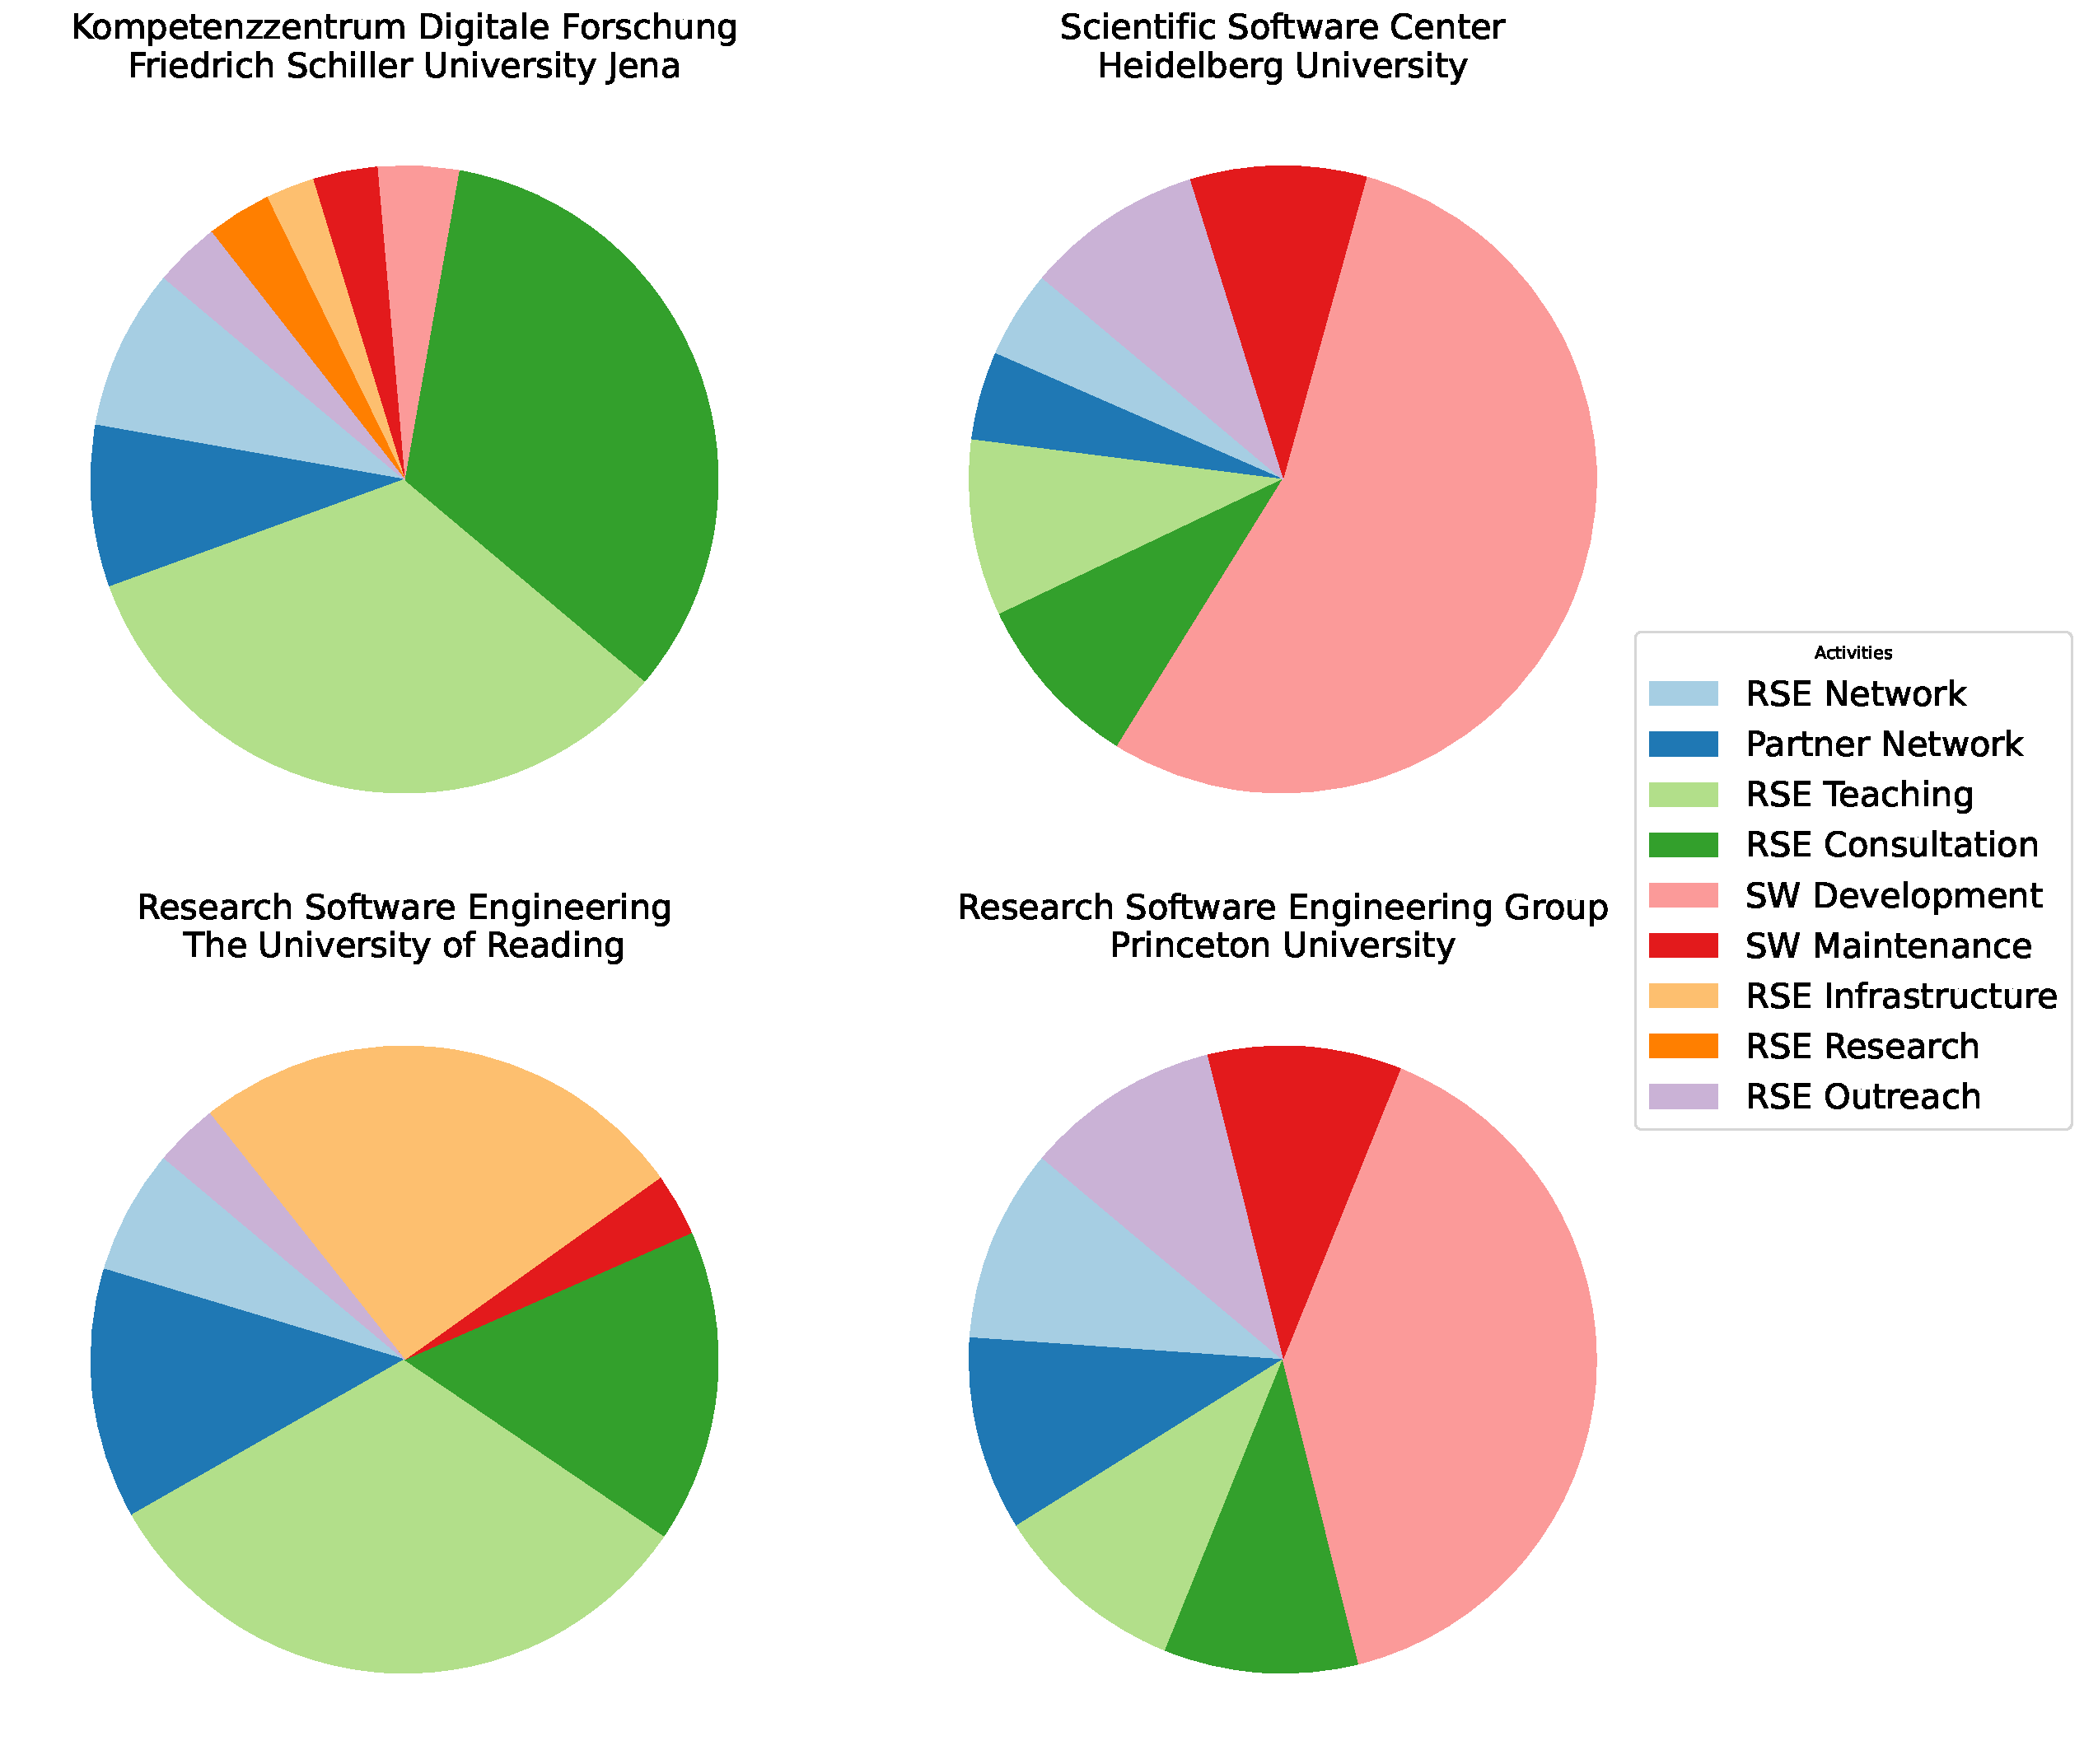
\includegraphics[width=.8\textwidth]{./group_composition_plot/group_composition_plot_the_fantastic_four.pdf}
\caption{National and international examples of RSE units and their service portfolio, structured by activities corresponding to the modules described in Section~\ref{sec:vision}.
  \protect\input{./group_composition_plot/group_composition_plot_the_fantastic_four.labels}\unskip.
  Heidelberg and Princeton offer development services, whereas Jena and Reading focus mostly on teaching and consultation services.}%
\label{fig:survey}
\end{figure}

A number of successful RSE units have already been established in Germany and many more exist in other countries, especially the UK and the US\@.
In order to understand the service portfolio of these existing RSE units, we conducted a small survey that received a total of twelve responses from Germany, the UK and the US\@.
We asked RSE units for the composition of their service portfolio --- the results are shown in Figure~\ref{fig:survey}.

From the gathered data and the additional free text information of the participants, we conclude that the service components that we have identified in Section~\ref{sec:vision} are indeed relevant for existing RSE units.
Additionally, we see a large diversity in the weighting of these components, which is to be expected given the different environments of the RSE units.
Within this diverse data set, we identified two rather different archetypes of RSE units: those that offer development services and those that do not.
The RSE units offering development services would typically invest a lot of their resources into this component, whereas others put a much larger emphasis on teaching and consultation services.
We should note however, that our survey did not collect information about the size of the RSE unit.
It is likely that the RSE units offering development services are also larger in size,
  and that their total resource commitment to teaching and consultation services is similar to that of those RSE units that do not offer development services.

When setting up a new RSE unit, it is important to find the best service portfolio composition for the local environment.
This depends on the demand by scientists at the institution, existing structures and the available funding.

\section{Realisation Strategy}%
\label{sec:realisation}

We propose building blocks for individual realisation strategies for central institutional RSE units.
We start by listing different possibilities for funding RSE positions at a research institution.
Following that, we describe a potential transition pathway, starting from existing structures that have grown in research alliances such as, \eg{} DFG-funded Collaborative Research Centres or also in research departments of an institution.
This is complemented by discussions of the possibility of outsourcing RSE services and of the challenging task of identifying and hiring suitable RSE candidates.

\subsection{Funding Sources}%
\label{sec:funding}

We see four basic options for financing RSE positions, which we will briefly explain below:
\begin{enumerate}
\item ordinary budget positions,
\item overhead of externally funded projects,
\item explicitly requested person-months in externally funded projects, and
\item dedicated RSE calls.
\end{enumerate}
While each option stands for itself, in reality, an institutional RSE unit will likely need to finance its staff by an appropriate mixture of possibly all four options.
The mixture at a particular institution depends heavily on the local conditions.

At research institutions, it is important to resolve the conflict between time-limited research funding and the need for permanent positions, the latter being required to remain competitive with industry when hiring highly-qualified RSEs.
Experience is also an essential component of software engineering, which makes long-term employment indispensable.
In principle, pooling of positions and funds makes it possible to finance permanent positions from changing and mixed sources.
An institution’s leadership has to justify taking the corresponding risk of failing to raise external funds.
\begin{enumerate}
\item It seems natural to allocate ordinary budget positions for RSEs.
      However, particularly at German universities, it is usually impossible to create completely new budget positions and the only feasible way is to rededicate an existing position after its corresponding holder has left.
      Depending on the local circumstances at an institution, this can be a cumbersome and time-consuming process for each such position.
\item Funding organisations additionally allocate a portion of the direct project funds as overhead, which is typically divided between the institution and the applicant.
      We propose using a small percentage of the overhead agglomerated at the institution to permanently finance central RSE positions.
      Assuming a third-party funding income of €50 million annually and a 20\% overhead, €100,000 in permanent funding requirements for one person-year would only account for 1\% of this overhead.
\item In project applications involving the development of research software, corresponding person-months should be requested to finance RSE tasks.
      In this way, an applicant can book a fixed number of working hours from the RSE pool and pay for the costs accordingly.
      This model has been successfully implemented at several UK universities.
      In order to scale, it needs to be supported by an institutional policy.
      Large scale collaborative projects can often apply for dedicated technical support positions that align well with the idea of RSE units.
      For example, the German Research Foundation allows requesting funding for “central service units or external service providers” in grant proposals aimed at developing research software~\autocite{katerbow_dfg_rse_2024}.
\item Funding organisations are increasingly recognising the need for sustainable research software development and are setting up correspondingly designated funding programmes.
      The DFG has already organised three calls for proposals in 2016~\autocite{DFGCall2016NachhaltigkeitFS}, 2019~\autocite{DFGCall2019Qualitaetssicherung}, and 2022~\autocite{DFGCall2022ResearchSoftware,katerbow_dfg_rse_funding_2018}.
      It is to be expected that even more programs will be launched in the future.
      An already established RSE unit at an institution increases the chances of being successful in such calls.
\end{enumerate}

In addition to these funding options, we encourage funding agencies to provide seed funding for the establishment of RSE structures.
Such seed grants ease the decision making process in organisations and give RSEs the leeway to establish collaborations with researchers without the direct need to ask for remuneration.

\subsection{Transition Pathway}

We propose a potential transition path, beginning with purely embedded RSEs---distributed across the institution and linked to individual research groups and their projects---and leading toward a centralised institutional RSE unit.
After starting with initial measures not necessarily requiring dedicated funding, we discuss developing a business plan and how the RSE unit can be established.
We conclude with measures for promoting its growth.

\subsubsection{Initial Measures}
The following measures initialise the two modules presented in \autoref{sec:network} and \autoref{sec:teaching}.
While dedicated funding certainly is beneficial already for this step, it is not strictly necessary.
Once the two measures are in place, they can be used to illustrate the need for institutional RSE activities and therefore support funding proposals.

\paragraph{Network of RSEs}
Forming a network of RSEs localised at an institution can be initiated by any existing RSE individual or group that is preferably already in contact with other RSEs at the institution.
An institutional dedicated mailing list, chat group, and possibly other communication platforms can be created and a request for participation can be circulated via institutional channels such as an employee newsletter.
First common events such as social gatherings or RSE-related seminar talks can be organised and announced via the communication platform.
If the initiative is geographically local, this process can be accompanied, facilitated and strengthened by founding a local de-RSE chapter\footnote{A list of existing chapters: \url{https://de-rse.org/chapter/}.}.
Such network-building has been successfully initiated and implemented at several German research institutions such as the German Aerospace Center and the Forchungszentrum Jülich.

\paragraph{Pooling of existing teaching materials and training offers}
Depending on local RSE efforts, teaching materials and associated training formats are likely to already exist, distributed over individual institutional groups.
With the established network, the materials can be pooled and joint training can be offered to a wider institutional audience.
This step can be facilitated and formalised by offering introductory courses with a recognised curriculum as provided by The Carpentries\footnote{Carpentry examples: \url{https://software-carpentry.org/lessons/}}
or CodeRefinery\footnote{CodeRefinery examples: \url{https://coderefinery.org/lessons/}}.

\subsubsection{Developing a Business Plan}
Decision processes at institutions usually require a business plan on which to base the decision on whether to establish an RSE unit.
The business plan should include an outline of the RSE unit, its responsibilities and offerings as a subset of the nine modules presented in \autoref{sec:vision}, the funding, and the resulting benefits for the institution and its researchers.

A crucial and sometimes difficult question is how to position the RSE unit within the institution’s organisational structure.
A canonical place would be a new subunit of an existing unit close to software, training services and computing such as the local or central IT unit or the library.
Since most institutions already have an RDM unit, it seems natural to add the RSE unit as a parallel structure.
Another choice for the parent unit, particularly at universities, is the faculty for computer science.
A key aspect for this decision is that the RSE unit must be able to work with all research groups at the institution, for which it needs to act independently and thus should not be absorbed by a larger unit.
Since it offers a unique view on challenges related to research software, a smartly placed RSE unit is able to serve as link between the individual research groups and other central institutional units.
Therefore, determining the best place may involve discussions with several stakeholders at the institution and can already be beneficial for creating a network of institutional partners, see the module described in \autoref{sec:partners}.

The business plan also needs to address funding for the RSE unit's initial staff.
We consider it necessary that there is a certain amount of base funding provided by the institution that covers a basic RSE unit because much RSE work is not project based.
While options can be drawn from the discussion above, specific ideas should be discussed beforehand with the decision makers.
In order to facilitate long-term growth of the RSE unit, an institutional policy for requesting person-months in externally funded projects dedicated to RSE should be established.

Another part of the business plan should be the governance structure of the RSE unit.
One of the decisions to be made is if the unit head is supposed to be part of the unit itself or if the unit will be headed by somebody outside of it.
Additionally, installing an advisory board can be proposed in the plan, recruiting from the prospective institutional partners.

\subsubsection{Establishing the Unit}
Once the business plan has been approved by the institution, the RSE unit can be established accordingly.
The initial staffing depends crucially on the local institutional conditions.
One promising possibility is to start with two positions.
The first position is an RSE coordinator who is the contact person for all embedded RSEs.
Among other things, they are also responsible for organising meetings, developing training programs and reporting to stakeholders.
The second position is a central RSE, responsible for providing selected services and infrastructure.
These core positions complement the network of RSEs as described in~\autoref{sec:network}.

Drawing from the business plan and considering the initial staff situation, a first task of the centrally-funded structure is to define a basic service portfolio according to the modules described in \autoref{sec:vision}.
In addition to the aforementioned networking and teaching activities, see~\autoref{sec:network} and \autoref{sec:teaching}, it seems natural to start with consultation, see~\autoref{sec:consultation},
  as this allows to evaluate the potential necessities for other services such as development, infrastructure provisioning, and maintenance.

An extension of the initial service portfolio for a larger target audience requires the acquisition of funding for further positions, see below.

The best RSE unit can easily become useless if other departments as well as RSEs outside the central hub do not know about it.
Therefore, communication and outreach activities as described in~\autoref{sec:outreach}, particularly connecting to entities within the institution, is of utmost importance at this stage.
Although the inception of the RSE unit will be announced once the business plan has been approved by the institution, communication across the RSE hub, the RSE network and other departments should be done on a regular basis.
Such a communication should facilitate collaboration among RSEs while also keeping non-RSEs in the loop.


\subsubsection{Growth of the Unit}

\paragraph{Acquisition of further funding}
The most promising possibilities to acquire further funding seem to be explicitly requesting person-months in externally funded projects and dedicated RSE calls, as discussed in \autoref{sec:funding}.
We believe that the credibility of a research proposal that is asking for RSE funds is greatly enhanced if the RSE unit is part of this proposal from the beginning.
Over time, more and more researchers and proposals are expected to follow the institutional policy such that a consistent stream of income can be generated.

\begin{mdframed}
\textbf{Success Story:} Founded in January 2017, the Research Computing department of Princeton University has experienced a tremendous growth from the initial two FTEs to a total of 18 FTEs in the span of five years~\autocite{Cosden2022a}.
This growth is based on a continuous influx of new funded projects once successful projects showcase the additional value of RSE services to researchers.
\end{mdframed}

\paragraph{Offering of additional services}
With the additionally acquired funds, the service portfolio of the RSE unit can be enhanced regarding the modules described in \autoref{sec:vision}.
Obviously, the selection of modules and their share in the overall portfolio depend on the services that have been applied for in the corresponding proposals.
As this is strongly connected to hiring persons with the required expertise, this has to be carefully planned, see also below.

\begin{mdframed}
\textbf{Success Story:} The Scientific IT Services of ETH Zurich (SIS) started in 2013 with a handful of members and has (as of March 2024) around 50 members.
In addition to HPC services, the group also offers RSE services in various areas.
These include the development of software applications for RDM, support in the development and improvement of scientific software or the long-term maintenance of software developed in research groups.
In addition, SIS offers services in the areas of data science, machine learning, bioinformatics, trusted compute environments, and training and consulting.
\end{mdframed}

\subsection{Outsourcing}

Another possibility for the realisation of local RSE Service providers is by forming a spin-off and pooling the RSE Skills into an external company, which has benefits but also drawbacks.
This is an idea that so far lacks examples but for completeness we list some of the advantages and disadvantages.
Among the most obvious benefits is that this enables the creation of contracts outside of the WissZeitVG.\@
This also widens the customer base of the RSE unit since the newly founded company may obtain contracts from industry.
If this company is backed/branded by the institution, this enables another possibility for an institution to interact with local companies.
This might open opportunities for employees to more freely move between industries and academia.
But there are drawbacks.
Since the company is now an entity external to the institution, the procurement guidelines (“Vergaberichtlinien”) have to be fulfilled, which could, \eg{} mean to publicly invite tenders in order to have a competitive procedure.
A company has to be profitable entity but this could be partly softened by founding a not-for-profit entity.
Moreover, during the outsourcing contract, there has to be a coordinator at both sides and the flow of information from the academic institution to the contracted company has to be established.
These are some examples of additional administrative overhead due to the interaction with external partners, and certain domains will have issues with ensuring data privacy in this collaboration.
Some of these issues might be legally alleviated by forming framework agreements between an institution and the company.
It is of particular importance to agree on requirements and handover criteria, including quality assurance and license specifications.
On top of these drawbacks, there are soft factors, like whether an external company is accepted by scientists.

\subsection{Staff Acquisition/People}

RSE units need to be staffed, but where do potential employees come from?
So far, researchers accidentally find themselves in the role of an RSE because they pursued software development as part of their research.
A more deliberate approach with specific RSE education may be necessary to train people in sufficient numbers for central RSE units.
Being an RSE should be a career worth aspiring to, just as any other profession, with a long-term perspective.
This is a topic covered by a separate paper~\autocite{goth_foundational_competencies_2024}, but we provide a brief summary here:

These RSEs will bring a diverse set of skills centred around the topics of research,
  digital tools, and team-based work and hence can easily offer the consulting services mentioned in the previous section and guide people to their implementation in their workgroups.
To fill gaps, the RSE unit can also maintain a roster of freelance workers.
In order to retain RSEs, it should be possible for them to become experts in a field and hence this should make this job more attractive to budding RSEs,
  in order to mitigate the problem that some will only see this job as a one-year stint after their PhD and then move on to something else.
To facilitate the retention of skilled people, industry has long identified education as an effective tool.
For RSEs, this should be helped by yet to be formed academic facilities that enable them to keep on learning skills after their first professional qualification, supported by the respective certification programs.
In the longer run, research software engineering should be integrated into the existing study programmes.
One option here is the creation of an RSE master as a specialisation for computer science or application-domain bachelor programmes.
This should be complemented by adding a minor in these application-domain study programs such as biology, music, engineering etc.\ to facilitate the communication between the corresponding two groups of RSEs.
There are already some master's programs available (\eg{} in Berlin, Munich, and Stuttgart), that develop this specialisation on top of a domain bachelor.
Moreover, data science curricula already exist and more are in the process of being created.
A curated and continuously updated list of these programs is available at~\cite{learnandteachlearn}.

\section{Conclusions}
\label{sec:conclusions}

In this paper, we have outlined a vision for central RSE units in research institutions, focusing particularly on the German research landscape.
We have proposed a modular framework for structuring the services of such units, identifying nine fundamental modules and providing concrete pathways for their implementation.
Our survey of existing RSE units illustrates that such structures can take various forms, ranging from consultation-focused groups to those offering extensive software development services.
Yet, all serve to consolidate expertise within a research institution, strengthen cooperation across scientific disciplines, and increase the overall quality of research.

Besides addressing local needs in software development and maintenance, well-established RSE units also bring broader institutional benefits, such as improved funding acquisition or enhanced reputational standing.
They further enable closer collaboration among related domains like HPC, data management, and digital infrastructure.
This ultimately leads to more sustainable, reproducible, and impactful research on and with software-based methods.

We encourage decision makers to strategically invest in and formalise central RSE units, recognising their role as indispensable partners in modern research environments.
By unifying previously scattered RSE efforts into a coordinated approach with clear mandates, stable funding, and long-term career prospects, institutions have the opportunity to significantly enhance their research capabilities and competitiveness in an increasingly digital scientific world.


\printbibliography[heading=bibintoc]

\end{document}
